%-------------------------------------------%
\section{ODE description of LTI systems}
%-------------------------------------------%
    \begin{figure}[H] 
        \centering
        % 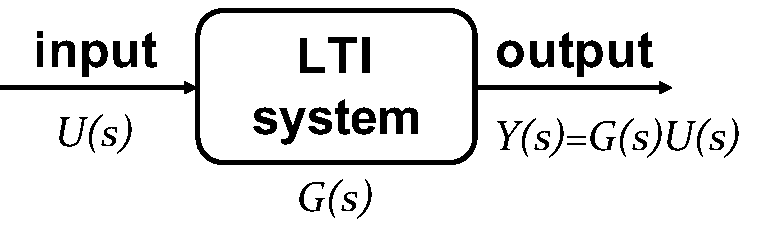
\includegraphics[width=0.4\textwidth]{images/LTI_independent.pdf}
        \begin{tikzpicture}[auto, node distance=2cm,>=latex',line width=1pt]
\centering
    \node [input, name = input] {};
    \node [block, right of = input] (controller) {LTI system};
    \node [output, right= 3.5cm of controller] (output) {};

    \draw [draw,->] node[below=.1cm] {$U(s)$} node[above=.1cm] {\textbf{input}}(input) --  (controller) node [below=.1cm of controller]{$G(s)$};
    \draw [->] (controller) -- node[below=.1cm] {$Y(s)= G(s)U(s)$} node[above=.1cm] {\textbf{output}} (output);
\end{tikzpicture}
        \caption{Linear time-invariant system}
    \end{figure}
    
\begin{itemize}
    \item LTI systems can be described by ODEs with constant coefficients in time domain:
        \[ a_{n} \frac{d^{n}y(t)}{dt^{n}}+...+a_{1} \frac{dy(t)}{dt}+a_{0} y(t) = b_{m} \frac{d^{m}u(t)}{dt^{m}}+...+b_{1} \frac{du(t)}{dt}+b_{0} u(t) \]

    \item Assuming there is zero initial conditions, take Laplace transform:
        \[ a_{n} s^{n} Y(s)+...+ a_{1} s Y(s) + a_{0} Y(s) = b_{m} s^{m} U(s)+...+b_{1} s U(s) + b_{0} U(s) \]
        \ where $\mathcal{L}[y(t)] = Y(s)$ and $\mathcal{L}[u(t)] = U(s)$. 

    \item \textbf{Transfer Function} is defined as:
        \[ \boxed{G(s)=\frac{Y(s)}{U(s)}=\frac{b_{m} s^{m}+...+b_{1} s +b_{0}}{a_{n} s^{n}+...+a_{1} s+a_{0}},\quad m \leq n }\] 
        
        \begin{itemize}
             \item Laplace transform of \textbf{output} divided by Laplace transform of \textbf{input}, assuming zero initial conditions.
             
             \item Ratio of polynomial in $s$.
             
             \item Transfer function is independent of the form of the input
        \end{itemize}
\end{itemize}
\ \\
\textbf{Properties of transfer functions:}
\begin{itemize}
    \item Linear functions
        \[ 
        G(s) (aU_{1}(s)+bU_{2}(s)) = aG(s)U_{1}(s)+b G(s) U_{2}(s)
        \]
    \item Commutative
        \[G_{1}(s) G_{2}(s) = G_{2}(s)G_{1}(s)\]
    \item Associative
        \[G_{1}(s) +G_{2}(s) = G_{2}(s) +G_{1}(s)\]
\end{itemize}

%---------------EXAMPLE START---------------%
\begin{ex}{Mass-Spring-Damper system}
    \begin{figure}[H] 
        \centering
        \begin{tikzpicture}[every node/.style={draw,outer sep=0pt,thick}]
    \tikzstyle{spring}=[thick,decorate,decoration={zigzag,pre length=0.3cm,post length=0.3cm,segment length=6}]
    \tikzstyle{damper}=[thick,decoration={markings,  
      mark connection node=dmp,
      mark=at position 0.5 with 
      {
        \node (dmp) [thick,inner sep=0pt,transform shape,rotate=-90,minimum width=15pt,minimum height=3pt,draw=none] {};
        \draw [thick] ($(dmp.north east)+(2pt,0)$) -- (dmp.south east) -- (dmp.south west) -- ($(dmp.north west)+(2pt,0)$);
        \draw [thick] ($(dmp.north)+(0,-5pt)$) -- ($(dmp.north)+(0,5pt)$) ; 
      }
    }, decorate]
    \tikzstyle{ground}=[fill,pattern=north east lines,draw=none,minimum width=0.75cm,minimum height=0.3cm]
    
    \node (M) [minimum width=1.5cm, minimum height=1.5cm] {$m$};
    \node (arrowstart) [name=arrowstart, above = 1cm of M.west,draw=none]{};
    \node (arrowend) [name=arrowend, above= 1cm of M.east,draw=none]{};
    
    \node (wall) [ground, rotate=-90, minimum width=1.5cm,yshift=-3cm] {};
    \draw (wall.north east) -- (wall.north west);
    
    % no need for ground, commented out
    % \node (gnd) [ground, rotate=0, minimum width=5cm,yshift=-0.9cm, xshift=-0.65cm] {};
    % \draw (wall.south east) -- (M.south east)--+(1.1cm,0);
    
    \draw [spring] (wall.160) -- ($(M.north west)!(wall.160)!(M.south west)$);
    \draw [damper] (wall.20) -- ($(M.north west)!(wall.20)!(M.south west)$);
    
    \draw [-latex,ultra thick] (M.east) ++ (0,0) -- +(1.1cm,0) node [above, draw=none]{$u(t)$} node [below=.15cm,draw=none]{Force};
    \draw [dashed] (M.east) ++ (0,0) -- +(0,1.5cm);
    \draw [-latex] (arrowstart) -- (arrowend) node[draw=none, above]{$y(t)$};
    
    \node[below=.3cm, draw=none] at (-2.1,-0.1){$c$};
    \node[above, draw=none] at (-2.1,0.5){$k$};
\end{tikzpicture}
    \end{figure}
    A Mass-Spring-Damper system can be characterized by ODE:
    \[ m\frac{d^{2}y(t)}{dt^{2}}+c\frac{dy(t)}{dt}+ky(t)=u(t) \]
    Take Laplace transform with zero initial condition:
    \[ ms^{2}Y(s)+csY(s)+kY(s)=(ms^{2}+cs+k)Y(s)=U(s) \]
    So the transfer function is 
    \[ G(s)=\frac{Y(s)}{U(s)}= \frac{1}{ms^{2}+cs+k} \]
    If m=6, c=5 and k=1, 
    \begin{itemize}
    \item to find the impulse response:
    \[ 
    Y(s) = G(s)U(s) = G(s) 
    = \frac{1}{6s^{2}+5s+1} 
    = \frac{-2}{2s+1}+\frac{3}{3s+1}= \frac{-1}{s+0.5}+\frac{1}{s+\frac{1}{3}} 
    \]
    \[ 
    y(t) = g(t) 
    = \mathcal{L}^{-1} [G(s)] 
    = -e^{-t/2}+-e^{-t/3} 
    \]
    
    \item to find the step response:
    \[
    Y(s) = G(s)U(s) = \frac{1}{s}\frac{1}{6s^{2}+5s+1} 
    = \frac{4}{2s+1}-\frac{9}{3s+1} +\frac{1}{s} 
    = \frac{2}{s+\frac{1}{2}}-\frac{3}{s+\frac{1}{3}} +\frac{1}{s} \]
    \[ y(t) = 2e^{-t/2}-3^{-t/3} +1 \]
    \end{itemize}
    
    \textbf{Comments:}
    \begin{itemize}
     \item From the example above, the solutions of denominator of the transfer function are $s = -\frac{1}{2}$ and $s = -\frac{1}{3}$;
     
     \item These two solutions are the \textbf{poles} of the system. 
     \item Poles define the long-time behaviours of the system: whether the system can stay at certain level, or converges to 0 or $\infty$.
     
     \item $s = -\frac{1}{2}$ and $s = -\frac{1}{3}$ are real, negative solutions, so as $t\to \infty$, 
     for step response,  $y(t) \to 1$, (and for impulse response, $y(t) \to 0$). They have no affect on long-term behaviour of the system.
    \end{itemize}
\end{ex}
%---------------EXAMPLE END---------------%

%-------------------------------------------%
\subsection{Zero-pole-gain}
%-------------------------------------------%
Transfer function can be written as:
\begin{align*}
\begin{split}
    G(s)
    &=\frac{Y(s)}{U(s)}=\frac{b_{m} s^{m}+...+b_{1} s +b_{0}}{a_{n} s^{n}+...+a_{1} s+a_{0}}\\
    &=\boxed{K\frac{(s-z_{1})(s-z_{2})...(s-z_{m})}{(s-p_{1})(s-p_{2})...(s-p_{n})}}\\
\end{split}
\end{align*}
\ where $K$ is the gain.

 \begin{itemize}
      \item Zeros $\{z_{1} , \ z_{2}, \ ..., \ z_{m}\}$ are the solutions of $N(s)=0$;
      \item Poles $\{p_{1} , \ p_{2}, \ ..., \ p_{n}\}$ are the solutions of $D(s)=0$;
 \end{itemize}

%---------------EXAMPLE START---------------%
\begin{ex}{}
Find the poles and zeros of a LTI system
    \[\frac{d^{2}y}{dx^{2}}+5\frac{dy}{dx}+6y = 2\frac{du}{dt}+u\]
\hrule
\vspace{.3cm}
\begin{enumerate}
    \item Obtain the transfer function by Laplace transform
        \[s^{2}Y(s)+5sY(s)+6Y(s) = 2sU(s)+U(s)\]
        This gives
        \[G(s) =\frac{Y(s)}{U(s)} = \frac{2s+1}{s^{2}+5s+6}\]
        
    \item Factorize the transfer function
        \begin{itemize}
            \item $2s+1=0$, zero at $s = -\frac{1}{2}$.
            \item $(s+3)(s+2)=0$, poles at $s = -2$ and $s = -3$
        \end{itemize}
\end{enumerate}
\end{ex}
%----------------EXAMPLE END----------------%
%---------------EXAMPLE START---------------%
\begin{ex}{}
Find the ODE representing the system with 
\begin{itemize}
    \item poles at $-1\pm 2j$
    \item zero at -4 
    \item gain factor 3
\end{itemize}
\hrule
\vspace{.3cm}
\begin{enumerate}
    \item Find the transfer function:
    \[
    G(s) = \frac{Y(s)}{U(s)} 
    = 3\frac{s-(-4)}{[s-(-1-2j)][s-(-1+2j)]} 
    = 3\frac{s+4}{s^{2}+2s+5}
    \]
    
    \item ODE can be found by taking Inverse Laplace transform:
    \[
    (s^{2}+2s+5)Y(s) = 3(s+4)U(s)
    \quad \xrightarrow{\mathcal{L}} \quad
    \frac{d^{2}y}{dt^{2}}+2\frac{dy}{dt}+5y 
    = 3\frac{du}{dt}+12u 
    \]
\end{enumerate}
\end{ex}
%----------------EXAMPLE END----------------%


%-------------------------------------------%
\subsection{Block Diagrams}
%-------------------------------------------%
Block diagrams are used to visually represent LTI systems.
\begin{figure}[H] \centering
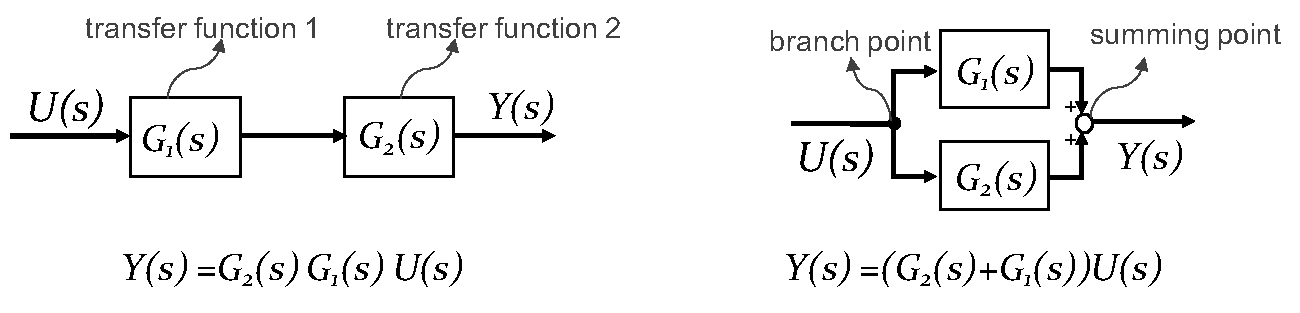
\includegraphics[width=.9\textwidth]{images/block_diagram.pdf}
\caption{Block diagram explanation}
\end{figure}

%---------------EXAMPLE START---------------%
\begin{ex}{}
Consider the simplest negative feedback system, as shown below. Find the transfer function of the system.
\begin{figure}[H] 
    \centering
    \begin{tikzpicture}[auto, node distance=2cm,>=latex',line width=1pt]
    \node [input, name=input] {};
    \node [sum, right of=input] (sum) {};
    \node [block, right of=sum] (controller) {$G(s)$};
    \coordinate [right of = controller, circle, scale=0.5, fill](tooutput){};
    \node [output, right of=tooutput] (output) {};
    \coordinate [below= 1.5cm of tooutput] (measurements) {};

    \draw [draw,->] (input) -- node {$U(s)$\ {\footnotesize$+$}} (sum); 
    \draw [->] (sum) -- node {} (controller);
    \draw [-] (controller) -- (tooutput);
    \draw [->] (tooutput) -- node[] {$Y(s)$} (output);
    \draw [-] (tooutput) |- (measurements);
    \draw [->] (measurements) -| 
    node[pos=1] {{\footnotesize$-$}} (sum);
\end{tikzpicture}
\end{figure}
\hrule \vspace{.3cm} 
\textit{Note:} \  the minus sign in the figure indicates the negative feedback in the system.
\[ Y(s) = G(s)(U(s)-Y(s))\]
Rearrange, then we find the transfer function of this closed-loop system:
\[\boxed{\frac{Y(s)}{U(s)} = \frac{G(s)}{1+G(s)}}\]
\end{ex}
%----------------EXAMPLE END----------------%
%---------------EXAMPLE START---------------%
\begin{ex}{} 
Derive the transfer function of the following negative feedback system.
\begin{figure}[H] 
    \centering
    \begin{tikzpicture}[auto, node distance=2cm,>=latex',line width=1pt]
    \node [input, name = input] {};
    \node [sum, right of = input] (sum) {};
    \node [block, right of = sum] (controller1) {$G_{1}(s)$};
    \node [sum, right = 0.9cm of controller1] (sum2) {};
    \node [block, right of= sum2] (controller2) {$G_{2}(s)$};
    \node [block, below= 0.5cm of controller2] (controller3) {$G_{3}(s)$};
    \coordinate [right of = controller2](right2con2){};
    \coordinate [right of = right2con2](tooutput){};
    \node [output, right of = tooutput] (output) {};
    \coordinate [below = 2cm of tooutput] (measurements) {};

    \draw [draw,->] (input) -- node {$U(s)$ \ {\footnotesize$+$}} (sum); 
    \draw [->] (sum) -- node {} (controller1);
    \draw [->] (controller1) -- node {{\footnotesize$+$}} (sum2) -- (controller2);
    \draw [-] (controller2) -- (right2con2) |- (controller3);
    \draw [->] (controller3) -| node[pos=1] {{\footnotesize$+$}}(sum2);
    \draw [-] (controller2) -- (tooutput);
    \draw [->] (tooutput) -- node[] {$Y(s)$} (output);
    \draw [-] (tooutput) |- (measurements);
    \draw [->] (measurements) -| 
    node[pos=1] {{\footnotesize$-$}} (sum);
\end{tikzpicture}
\end{figure}
\hrule \vspace{.3cm} 
Consider the dashed section: 
\begin{figure}[H] 
    \centering
    % 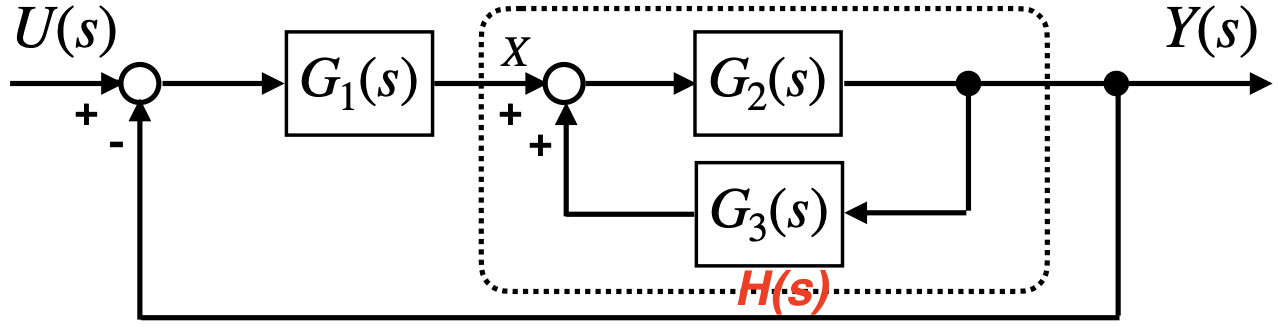
\includegraphics[width=.5\textwidth]{images/BD2_dashed.png}
    \begin{tikzpicture}[auto, node distance=2cm,>=latex',line width=1pt]
    \node [input, name = input] {};
    \node [sum, right of = input] (sum) {};
    \node [block, right of = sum] (controller1) {$G_{1}(s)$};
    \node [sum, right = 0.9cm of controller1] (sum2) {};
    \node [block, right of= sum2] (controller2) {$G_{2}(s)$};
    \node [block, below= 0.5cm of controller2] (controller3) {$G_{3}(s)$};
    \coordinate [right of = controller2, circle, scale=0.5, fill](right2con2){};
    \coordinate [right of = right2con2, circle, scale=0.5, fill](tooutput){};
    \node [output, right of = tooutput] (output) {};
    \coordinate [below = 2cm of tooutput] (measurements) {};

    \draw [draw,->] (input) -- node {$U(s)$ \ {\footnotesize$+$}} (sum); 
    \draw [->] (sum) -- node {} (controller1);
    \draw [->] (controller1) -- node {{\footnotesize$+$}} (sum2) -- (controller2);
    \draw [-] (controller2) -- (right2con2) |- (controller3);
    \draw [->] (controller3) -| node[pos=1] {{\footnotesize$+$}}(sum2);
    \draw [-] (controller2) -- (tooutput);
    \draw [->] (tooutput) -- node[] {$Y(s)$} (output);
    \draw [-] (tooutput) |- (measurements);
    \draw [->] (measurements) -| 
    node[pos=1] {{\footnotesize$-$}} (sum);
    
    \draw[red, dashed] ([xshift=-3mm, yshift=5mm]sum2.west) -- ([xshift=3mm, yshift=5mm]right2con2.east) |- ([yshift=-3mm]controller3.south) -| node[left]{$H(s)$} ([xshift=-3mm, yshift=5mm]sum2.west);
\end{tikzpicture}
\end{figure}
The transfer function of the dashed section, $H(s)$, that is equivalent to the combination of $G_{2}(s)$ and $G_{3}(s)$.
\begin{itemize}
    \item Let the input to the dashed section be $X(s)$:
        \[Y(s) = G_{2}(s)(X+G_{3}(s)Y(s))\]
    \item Rearrange:
        \[
        H(s) = \frac{Y(s)}{X(s)} = \frac{G_{2}(s)}{1-G_{2}(s)G_{3}(s)}
        \]
\end{itemize}
Then we are going to find the equivalent transfer function to the whole system:
\[Y(s) =(U(s)-Y(s))G_{1}(s)H(s)\]
This gives us the final result:
\[
T.F. \ = \ 
\frac{Y(s)}{U(s)} = 
\frac{G_{1}(s)H(s)}{1+G_{1}(s)H(s)}, \quad \text{where} \ 
H(s) = \frac{G_{2}(s)}{1-G_{2}(s)G_{3}(s)}
\]
\end{ex}
%----------------EXAMPLE END----------------%